\chapter{Results\label{chap:result}}

    In this chapter, we present the results of experiments conducted and provide answers to all research questions from Section~\ref{sec:RQs}. Section~\ref{sec:results_rq1} takes up the majority of this chapter and addresses results achieved on the task of \emph{Expertise Extraction}. Analysis results of \emph{Cross-Platform Expertise} are presented in Section~\ref{sec:results_rq2}, while \emph{Cross-Platform Transferable Knowledge} results are reported in Section~\ref{sec:results_rq3}.  Section~\ref{sec:results_rq4} presents our results and conclusions for \emph{Expertise Evolution}.

    \section{Expertise Extraction\label{sec:results_rq1}}
        % RQ1: How to extract the major expertise areas of Stack Overflow and GitHub users? How do expertise trends compare on Stack Overflow and GitHub?
        
       For the Expertise Extraction task \emph{three} novel techniques have been proposed: Baseline LDA Based Expertise Extraction \emph{(Technique 1)}, Improved LDA Based Expertise Extraction \emph{(Technique 2)}, and Pre-trained Word2Vec Based Expertise Extraction \emph{(Technique 3)}. Technique 2 and Technique 3 have two different variations each: the first one is using \emph{Average-pooling}, while the second one is using the \emph{Max-pooling} technique for down-sampling. Including these two variations, a total of five models are considered:
        
        \Edited{Fixed names of the techniques in results}
        
        \begin{itemize}
            \item Model 1: Baseline LDA Based Expertise Extraction, labelled as \emph{B\_LDA},
            \item Model 2: Improved LDA Based Expertise Extraction obtained by Average-pooling, labelled in tables as \emph{LDA\_AVG},
            \item Model 3: Improved LDA Based Expertise Extraction obtained by Max-pooling, labelled in tables as \emph{LDA\_MAX},
            \item Model 4: Pre-trained Word2Vec Based Expertise Extraction obtained by Average-pooling, labelled in tables as \emph{W2V\_AVG},
            \item Model 5: Pre-trained Word2Vec Based Expertise Extraction obtained by Max-pooling, labelled in tables as \emph{W2V\_AVG}.
        \end{itemize}
        
        The above listed five models are evaluated against a baseline (naive) model (see Section~\ref{subsec:random_model}), which is a frequency-based random model. When evaluating the extraction of expertise areas, two similar experiments were used. In the first experiment, each model's performance is evaluated against the ground truth knowledge from Section \ref{sec:expertise_survey} with the specification that a model has to output exactly as many expertise terms as the ground truth annotation contains. This case is referred to as Experiment 1. In the second experiment, each model is evaluated against the ground truth annotation, but there are no restrictions applied to the number of expertise terms to be returned by each model. In this scenario, the models can be more robust, as they can return all the expertise terms found by the underlying algorithm, without needing to rank and return only the top-$n$ expertise terms. Throughout this chapter, this more robust, less restrictive experiment setup will be referred to as Experiment 2. Furthermore, each one of the above mentioned experiments has to variations: expertise extraction from 1) GitHub data (labelled Experiment \emph{A}) and 2) Stack Overflow data (labelled Experiment \emph{B}).
        
        \subsection{Experiment 1}
        
            Table~\ref{tab:GH_results1} shows the top-$3$ highest evaluation metric scores for each one of the five models from \emph{Experiment 1A} - Expertise Extraction from GitHub Data. The top-$3$ ranking is done based on the highest cosine similarity scores. The five models are compared against a frequency-based random model (referred to as \emph{Baseline}), whose evaluation metrics comes from averaging the results of 10,000 random samples.
            
            \begin{table}
              \centering
              \caption{Results of Experiment 1A - Expertise Extraction from GitHub Data.}\label{tab:GH_results1}
                \vspace{6pt} % Required to get proper spacing between caption and table
                \resizebox{\textwidth}{!}{
              \begin{tabular}{|c|c|c|c|c|c|c|c|}
                \hline
                \thead{Top 3\\Results}& \diaghead{\theadfont DiagonalHead}{Metrics}{Model} &
                \thead{\textbf{B\_LDA}} & \thead{\textbf{LDA\_AVG}} & \thead{\textbf{LDA\_MAX}} & \thead{\textbf{W2V\_AVG}} & \thead{\textbf{W2V\_MAX}} & \thead{\textbf{Baseline}}\\
                \hline
                \multirow{3}*{1} & Cosine Sim. & 0.6690 & 0.7187 & 0.7357 & \textbf{0.7998} & 0.7317 & 0.5962 \\
                      & Jaccard Sim. & 0.0658 & 0.0751 & 0.1040 & 0.0765 & 0.1049 & 0.0286 \\
                      & BLEU Score & 0.1197 & 0.1340 & 0.1767 & 0.1368 & 0.1782 & 0.0540 \\
                \hline
                \multirow{3}*{2} & Cosine Sim. & 0.6689 & 0.7183 & 0.7351 & 0.7959 & 0.7316 & 0.5962 \\
                       & Jaccard Sim. & 0.0658 & 0.0750 & 0.1037 & 0.0818 & 0.1049 & 0.0286 \\
                       & BLEU Score & 0.1197 & 0.1338 & 0.1762 & 0.1452 & 0.1782 & 0.0540 \\
                \hline
                \multirow{3}*{3} & Cosine Sim. & 0.6683 & 0.7183 & 0.7351 & 0.7959 & 0.7316 & 0.5962 \\
                       & Jaccard Sim. & 0.0652 & 0.0750 & 0.1037 & 0.0818 & 0.1049 & 0.0286 \\
                       & BLEU Score & 0.1186 & 0.1338 & 0.1762 & 0.1452 & 0.1782 & 0.0540 \\
              \hline 
            \end{tabular}}
            \end{table}
            
            The results from Table~\ref{tab:GH_results1} indicate that each model's top-$3$ highest evaluation scores outperform the baseline model's each one of the three metrics. \emph{W2V\_AVG}, which is named \emph{Expertise Extraction using Pre-trained Word2Vec based User and Topic Embeddings obtained by Average-pooling} achieves the highest cosine similarity score (\emph{0.7998}). The baseline cosine similarity score of the random model is \emph{0.5962}. Jaccard similarity and BLEU score are also reported, but cosine similarity is considered the primary evaluation metric when comparing different techniques' performance, due to the reasons explained in Section~\ref{sec:eval_expertise_prediction}. \emph{B\_LDA} is performing the worst, having its best cosine similarity score of \emph{0.6690}, and that is expected, since it is a topic probability distribution based technique, and does not use user and topic embeddings. \emph{LDA\_MAX} and \emph{W2V\_MAX} are performing very similarly, both plateauing around a cosine similarity score of \emph{0.73}. \emph{LDA\_AVG} performs a little worse than  \emph{LDA\_MAX} and \emph{W2V\_MAX} by having the maximum cosine similarity score of \emph{0.7187}. 
            
            It is difficult to understand how accurate these techniques are only based on cosine similarity scores obtained from calculating the semantic similarity between the bag of words of human annotations and model extraction. To illustrate different levels of semantic similarity of cosine similarity scores Table~\ref{tab:cos_sim} contains examples of term-pairs and their respective cosine similarity scores. These cosine similarity scores were obtained using the same pre-trained Word2Vec model\cite{efstathiou2018word} used in Section \ref{word2vec_model}. 
            
            \begin{table}
                  \centering
                  \caption{Example of Cosine Similarity Scores between Term-Pairs.} \label{tab:cos_sim}
                  \vspace{6pt} % Required to get proper spacing between caption and table
                  \resizebox{\textwidth}{!}{
                  \begin{tabular}{|c c c|c c c|}
                    \hline
                    Term 1 & Term 2 & Cosine Similarity & Term 1 & Term 2 & Cosine Similarity \\
                    \hline
                    php & python & 0.2529 & html & javascript & 0.6024 \\
                    java & python & 0.3929 & ajax & jquery & 0.6315 \\
                    analysis & visualization & 0.4524 & sklearn & tensorflow & 0.6858 \\ 
                    nodejs & reactjs & 0.4909 & bagging & random-forest & 0.7251 \\
                    java & jdk & 0.5517 & mysql & postgresql & 0.7997 \\
                    xml & json & 0.5866 & keras & tensorflow & 0.8391 \\
                    \hline
                  \end{tabular}}
            \end{table}
            
            Based on the sample cosine similarity scores from Table~\ref{tab:cos_sim} one can say that \emph{W2V\_AVG}'s best model extracts expertise terms with similar semantic similarity level to the contextual similarity between the `mysql' and `postgresql' term-pair. Likewise, \emph{LDA\_AVG}, \emph{LDA\_MAX} and \emph{W2V\_MAX} extract expertise terms with similar semantic similarity level to `random-forest' and `bagging' term-pair, while \emph{B\_LDA}'s best cosine similarity score classifies its semantic similarity level just below `tensorflow' and `sklearn' term-pair's. One could argue that the above mentioned semantic similarity levels correspond to contextually similar software engineering related word associations, thus illustrating that Table~\ref{tab:GH_results1}'s results lead to high levels of semantic similarity between the bags of words of human annotations and expertise terms extracted by the models.
            
            Unfortunately, as far as we are aware, the same kind of representation of similarity levels can not be easily created for \emph{Jaccard Similarities} and \emph{BLEU Scores}. Jaccard similarity is a measure of set similarity, and it highly depends not only on the magnitude of the set intersection, but the set union as well. BLEU score values range between 0 and 1, and the inventors of BLEU score report that in their study a professional human translator was able to achieve a score of \emph{0.3468} calculated against four reference annotations and \emph{0.2571} against two reference annotations\cite{papineni2002bleu}.
        
            Table~\ref{tab:GH_params1} found in Appendix \ref{appendix:model_params} contains all major parameters used to fit the models outlined in Table~\ref{tab:GH_results1}. The models were fitted using a hyper-parameter optimization process described in Section~\ref{sec:hyper-parameter_selection} and their parameters come from the parameter search space defined in Section~\ref{sec:hyper-parameter_selection}. Table~\ref{tab:GH_params1} suggests a general pattern of the GitHub data containing a relatively small number of topics: 10 in \emph{LDA\_AVG}, 11 being the most popular in \emph{B\_LDA}, \emph{LDA\_MAX} \& \emph{W2V\_MAX}, and 16 in the superior \emph{W2V\_AVG}. The parameter $\beta$ highly varies between 0.001, 0.005, 0.01 and 0.05, but in most cases $\beta=0.005$.
            
            Table \ref{tab:expertise_extractions} offers \emph{good, very good and bad} examples of actual expertise terms extracted by our models during Experiment \emph{1A}, compared with the ground truth human annotations. The expertise terms that are common across human annotation and model extraction are shown in \textbf{bold}. Alongside the expertise terms, the number of terms matched and the cosine similarity between the two bags of words are also reported in Table \ref{tab:expertise_extractions}. This type of expertise terms comparison demonstrates that Experiment \emph{1A}'s results lead to high levels of semantic similarity between the bags of words of human annotations and expertise terms extracted by the models.
        
            \begin{table}
              \centering
              \caption{Sample Annotation and Model Extraction Comparison from Experiment \emph{1A}.} \label{tab:expertise_extractions}
                \vspace{6pt} % Required to get proper spacing between caption and table
                 \resizebox{\textwidth}{!}{
                \begin{tabular}{|p{2cm}|p{5cm}|p{5cm}|p{1cm}|p{1cm}|}
                    \hline
                    Type of Example & Human Annotation & Model Extraction & Match & Cosine Sim.\\
                    \hline
                    Bad & [ui, linux, images, books, perl, c, data\_process, proxy, blogs, python, go, shell, c\#, javascript, web, maintaining, creating, java, css, html, dockerfile, image\_process, software, libraries, docker, ruby, tex, c++, groovy, writing, \textbf{development}, makefile, agile] & [php, wordpress, laravel, bundle, symfony, drupal, wp, framework, plugin, magento, composer, doctrine, symfony2, api, extension, redmine, simple, phpunit, library, cms, module, zend, p, form, admin, standards, integration, skeleton, silex, documentation, guzzle, custom, \textbf{development}] & 1/33 & 0.5361 \\ 
                    Good & [tls, programming, oss\_fuzz, c, bcyrpt, go, security, ssl, \textbf{rust}, \textbf{java}, homebrew, urllib3, \textbf{python}, software\_engineering, objective\_c, \textbf{ruby}, azure, powershell, \textbf{shell}, infra, propery\_base\_testing, cryptography, networking, makefile, html, open\_ssl, cpython, algorithms, \textbf{clojure}, vorbis]  & [\textbf{python}, \textbf{ruby}, php, scala, emacs, \textbf{clojure}, javascript, haskell, emacs\_lisp, c, \textbf{rust}, \textbf{java}, perl, spring, c++, rails, docker, mode, \textbf{shell}, r, ansible, awesome, elm, react, django, grails, elixir] & 6/30 & 0.7749 \\
                    Very Good & [objective\_c, type, go, css, typescript, \textbf{dockerfile}, \textbf{java}, \textbf{scala}, \textbf{python}, \textbf{ruby}, \textbf{javascript}, \textbf{shell}, \textbf{php}, \textbf{haskell}, script, swift, \textbf{c++}, smarty, html, \textbf{django}, \textbf{clojure}, vim\_script]  & [\textbf{python}, \textbf{ruby}, \textbf{php}, \textbf{scala}, \textbf{clojure}, \textbf{javascript}, \textbf{haskell}, c, rust, \textbf{java}, perl, spring, \textbf{c++}, rails, \textbf{docker}, \textbf{shell}, r, ansible, awesome, elm, react, \textbf{django}] & 12/22 & 0.9138  \\
                    \hline
                \end{tabular}}
            \end{table}
            
            Table~\ref{tab:SO_results1} shows the top-$3$ highest evaluation metric scores for each one of the five models from \emph{Experiment 1B} - Expertise Extraction from Stack Overflow Data. Same as before, the top-$3$ models are ranked based on the highest cosine similarity scores, and the models are compared against a \emph{Baseline}.
            
            \begin{table}
              \centering
              \caption{Results of Experiment 1B - Expertise Extraction from Stack Overflow Data.} \label{tab:SO_results1}
                \vspace{6pt} % Required to get proper spacing between caption and table
                \resizebox{\textwidth}{!}{
              \begin{tabular}{|c|c|c|c|c|c|c|c|}
                \hline
                \thead{Top 3\\Results}& \diaghead{\theadfont DiagonalHead}{Metrics}{Model} &
                \thead{\textbf{B\_LDA}} & \thead{\textbf{LDA\_AVG}} & \thead{\textbf{LDA\_MAX}} & \thead{\textbf{W2V\_AVG}} & \thead{\textbf{W2V\_MAX}} & \thead{\textbf{Baseline}}\\
                \hline
                \multirow{3}*{1} & Cosine Sim. & 0.5044 & 0.5582 & \textbf{0.5837} & 0.5607 & 0.5820 & 0.3721 \\
                      & Jaccard Sim. & 0.0160 & 0.0406 & 0.0435 & 0.0320 & 0.0556 & 0.0104 \\
                      & BLEU Score & 0.0313 & 0.0770 & 0.0823 & 0.0612 & 0.1041 & 0.0199 \\
                \hline
                \multirow{3}*{2} & Cosine Sim. & 0.4997 & 0.5560 & 0.5717 & 0.5574 & 0.5746 & 0.3721 \\
                      & Jaccard Sim. & 0.0295 & 0.0747 & 0.0814 & 0.0404 & 0.0784 & 0.0104 \\
                      & BLEU Score & 0.0560 & 0.1366 & 0.1471 & 0.0768 & 0.1424 & 0.0199 \\
                \hline
                \multirow{3}*{3} & Cosine Sim. & 0.4755 & 0.5409 & 0.5676 & 0.5537 & 0.5736 & 0.3721 \\
                      & Jaccard Sim. & 0.0127 & 0.0754 & 0.0821 & 0.0718 & 0.0305 & 0.0104 \\
                      & BLEU Score & 0.0247 & 0.1366 & 0.1478 & 0.1312 & 0.0584 & 0.0199 \\
              \hline 
            \end{tabular}}
            \end{table}
            
            The results from Table~\ref{tab:SO_results1} show that each model's top-$3$ highest evaluation scores outperform the baseline model on each one of the three metrics. \emph{LDA\_MAX}, which is named Expertise Extraction using LDA based User and Topic Embeddings obtained by Max-pooling achieves the highest cosine similarity score (\emph{0.5837}), thus it can be considered the superior technique on the Stack Overflow data set. The baseline cosine similarity score of the random model is \emph{0.3721}, which is much lower than all other model's cosine similarity scores. \emph{B\_LDA} is performing the worst, having its best cosine similarity score of \emph{0.5044}. \emph{LDA\_AVG} and \emph{W2V\_AVG} are performing very similarly, both plateauing close to a cosine similarity score of \emph{0.56}. \emph{W2V\_MAX} is a very close second by having a maximum cosine similarity score of \emph{0.5820}, and barely being outperformed by the superior \emph{LDA\_MAX}.
            
            The results of Table~\ref{tab:SO_results1} show a trend of \emph{LDA\_MAX} and \emph{W2V\_MAX} outperforming \emph{LDA\_AVG} and \emph{W2V\_AVG}. This means that performing down-sampling using Max-pooling, instead of Average-pooling seems to work better on the Stack Overflow data set, which was not the case in Experiment 1A conducted on the GitHub data set.
            
            Sample cosine similarity scores from Table~\ref{tab:cos_sim} can help associate semantic similarity levels to the results presented in Table~\ref{tab:SO_results1}. Based on Table~\ref{tab:cos_sim} one can say that  \emph{LDA\_MAX} and \emph{W2V\_MAX}'s best models extract expertise terms with similar semantic similarity level to the contextual similarity between the `xml' and `json' term-pair. Likewise, \emph{LDA\_AVG} and \emph{W2V\_AVG} extract expertise terms with similar semantic similarity level to `java' and `jdk' term-pair, while \emph{B\_LDA}'s best cosine similarity score classifies its semantic similarity level just above `nodejs' and `reactjs' term-pair's. The above mentioned term-pairs correspond to contextually similar software engineering related word associations with similar semantic similarity levels to the model performances in Table~\ref{tab:SO_results1}. Thus, one could argue that Table~\ref{tab:SO_results1}'s results lead to high levels of semantic similarity between the bags of words of human annotations and expertise terms extracted by the models.
            
            Table~\ref{tab:SO_params1} found in Appendix \ref{appendix:model_params} contains all major parameters used to fit the models outlined in Table~\ref{tab:SO_results1}. Table~\ref{tab:SO_params1} suggests a general pattern of the Stack Overflow data containing a relatively large number of topics: \{40,29,45\} in  \emph{B\_LDA}, and \emph{LDA\_AVG} and \emph{LDA\_MAX} have 33 \& 27 number of topics in common, while \emph{W2V\_AVG} and \emph{W2V\_MAX} have 48 \& 31 number of topics in common. The most common number of topics out of the best performing models is 27. The parameter $\beta$ highly varies between 0.01, 0.1, 0.5 and 1, but in most cases $\beta=1$.
        
        \subsection{Experiment 2}
            The results of Experiment \emph{2A} and \emph{2B} can be seen in Table \ref{tab:GH_results2} and Table \ref{tab:SO_results2}. Note that Experiment \emph{2A} and \emph{2B} have no restrictions applied to the number of expertise terms returned by each model, thus the model will return as many expertise terms as it can find. This stipulation will significantly disadvantage the performance of Jaccard similarity and BLEU score (since the ratios change), but theoretically, it could increase the cosine similarity scores. 
            
            \begin{table}
              \centering
              \caption{Results of Experiment 2A - Expertise Extraction from GitHub Data.}\label{tab:GH_results2}
                \vspace{6pt} % Required to get proper spacing between caption and table
                \resizebox{\textwidth}{!}{
              \begin{tabular}{|c|c|c|c|c|c|c|c|}
                \hline
                \thead{Top 3\\Results}& \diaghead{\theadfont DiagonalHead}{Metrics}{Model} &
                \thead{\textbf{B\_LDA}} & \thead{\textbf{LDA\_AVG}} & \thead{\textbf{LDA\_MAX}} & \thead{\textbf{W2V\_AVG}} & \thead{\textbf{W2V\_MAX}} & \thead{\textbf{Baseline}}\\
                \hline
                \multirow{3}*{1} & Cosine Sim. & 0.6828 & 0.7377 & 0.7602 & \textbf{0.7761} & 0.7680 & 0.5962 \\
                      & Jaccard Sim. & 0.0246 & 0.0218 & 0.0251 & 0.0209 & 0.0144 & 0.0286 \\
                      & BLEU Score & 0.0277 & 0.0245 & 0.0279 & 0.0212 & 0.0127 & 0.0540 \\
                \hline
                \multirow{3}*{2} & Cosine Sim. & 0.6827 & 0.7364 & 0.7598 & 0.7750 & 0.7672 & 0.5962 \\
                       & Jaccard Sim. & 0.0249 & 0.0256 & 0.0254 & 0.0204 & 0.0138 & 0.0286 \\
                       & BLEU Score & 0.0281 & 0.0292 & 0.0288 & 0.0208 & 0.0122 & 0.0540 \\
                \hline
                \multirow{3}*{3} & Cosine Sim. & 0.6821 & 0.7362 & 0.7595 & 0.7748 & 0.7671 & 0.5962 \\
                       & Jaccard Sim. & 0.0241 & 0.0244 & 0.0259 & 0.0218 & 0.0131 & 0.0286 \\
                       & BLEU Score & 0.0271 & 0.0278 & 0.0295 & 0.0222 & 0.0116 & 0.0540 \\
              \hline 
            \end{tabular}}
            \end{table}
            
            Experiment \emph{2A}'s results from Table~\ref{tab:GH_results2} show that each model's top-$3$ highest cosine similarity scores outperform the baseline model's score. Unfortunately, that is not the case with Jaccard similarity and BLEU score, as these two metrics have decreased, even below the baseline model's performance. Oddly, this makes sense, as both of these metrics are ratios, which get affected by having no restrictions applied to the number of expertise terms returned by each model. For example, Jaccard similarity is calculated by dividing the cardinality of the set intersection with the cardinality of the set union. Having applied no restrictions to the number of expertise terms returned by the model, the set union increases drastically, and as a consequence Jaccard similarity scores have decreased. Same as for Experiment 1, when comparing different techniques' performance cosine similarity is considered the primary evaluation metric, due to the reasons explained in Section~\ref{sec:eval_expertise_prediction}.
            
            Interpreting the results from Table~\ref{tab:GH_results2} one can see that \emph{W2V\_AVG}, i.e.,  Expertise Extraction using Pre-trained Word2Vec based User and Topic Embeddings obtained by Average-pooling, achieves the highest cosine similarity score (\emph{0.7761}), thus it can be considered the superior technique on the GitHub data set, as this was the case in Experiment \emph{1A} as well. The baseline cosine similarity score of the random model is \emph{0.5962}. \emph{B\_LDA} is the worst performing model, but it improved its best cosine similarity score from \emph{0.6690} on Experiment \emph{1A} to \emph{0.6828} on Experiment \emph{2A}. This model having a low performance is no surprise, since \emph{B\_LDA} is a topic probability distribution based model which does not use user and topic embeddings. \emph{LDA\_MAX} and \emph{W2V\_MAX} are performing very similarly, both plateauing around a cosine similarity score of \emph{0.76}, which is higher than the score of \emph{0.73} achieved by both models in Experiment \emph{1A}. \emph{LDA\_AVG} performs a little worse than \emph{LDA\_MAX} and \emph{W2V\_MAX} by having a maximum cosine similarity score of \emph{0.7377}, which is still an improvement from \emph{0.7187} in Experiment \emph{1A}.
            
            Based on the examples of semantic similarity levels from Table~\ref{tab:cos_sim} one can say that \emph{W2V\_AVG}'s best model extracts expertise terms very close to the semantic similarity level between `mysql' and `postgresql' term-pair. In addition, \emph{LDA\_AVG} extract expertise terms with similar semantic similarity level to `random-forest' and `bagging'. Furthermore, \emph{B\_LDA}'s best cosine similarity score from Experiment \emph{2A} classifies its semantic similarity level similar to the term-pair of `tensorflow' and `sklearn'. These semantic similarity levels correspond to contextually similar software engineering related word associations, which strongly suggest that Table~\ref{tab:GH_results2}'s results lead to high levels of semantic similarity between the bags of words of human annotations and expertise terms extracted by the models.
             
            Table~\ref{tab:GH_params2} found in Appendix \ref{appendix:model_params} contains all major parameters used in the hyper-parameter optimization when fitting the models outlined in Table~\ref{tab:GH_results2}. The best models suggest a general pattern of the GitHub data containing a relatively small number of topics: 11 in \emph{B\_LDA}, 16 being the most popular in \emph{LDA\_MAX}, \emph{W2V\_AVG} \& \emph{W2V\_MAX}, while a surprising 21 in \emph{LDA\_AVG}. The parameter $\beta$ highly varies between 0.001, 0.005, 0.01 and 0.05, but in most cases it is either $\beta=0.001$ or $\beta=0.005$.
            
            \begin{table}
              \centering
              \caption{Results of Experiment 2B - Expertise Extraction from Stack Overflow Data.} \label{tab:SO_results2}
                \vspace{6pt} % Required to get proper spacing between caption and table
                \resizebox{\textwidth}{!}{
              \begin{tabular}{|c|c|c|c|c|c|c|c|}
                \hline
                \thead{Top 3\\Results}& \diaghead{\theadfont DiagonalHead}{Metrics}{Model} &
                \thead{\textbf{B\_LDA}} & \thead{\textbf{LDA\_AVG}} & \thead{\textbf{LDA\_MAX}} & \thead{\textbf{W2V\_AVG}} & \thead{\textbf{W2V\_MAX}} & \thead{\textbf{Baseline}}\\
                \hline
                \multirow{3}*{1} & Cosine Sim. & 0.5263 & 0.5361 & 0.5837 & \textbf{0.5902} & 0.5117 & 0.3721 \\
                      & Jaccard Sim. & 0.0099 & 0.0230 & 0.0435 & 0.0295 & 0.0102 & 0.0104 \\
                      & BLEU Score & 0.0117 & 0.0231 & 0.0822 & 0.0363 & 0.0087 & 0.0199 \\
                \hline
                \multirow{3}*{2} & Cosine Sim. & 0.5080 & 0.5304 & 0.5717 & 0.5821 & 0.5087 & 0.3721 \\
                      & Jaccard Sim. & 0.0223 & 0.0175 & 0.0816 & 0.0196 & 0.0120 & 0.0104 \\
                      & BLEU Score & 0.0267 & 0.0196 & 0.1471 & 0.0222 & 0.0101 & 0.0199 \\
                \hline
                \multirow{3}*{3} & Cosine Sim. & 0.5036 & 0.5266 & 0.5697 & 0.5698 & 0.5086 & 0.3721 \\
                      & Jaccard Sim. & 0.0111 & 0.0149 & 0.0303 & 0.0180 & 0.0106 & 0.0104 \\
                      & BLEU Score & 0.0136 & 0.0169 & 0.0579 & 0.0180 & 0.0090 & 0.0199 \\
              \hline 
            \end{tabular}}
            \end{table}
            
            Experiment \emph{2B}'s results from Table~\ref{tab:SO_results2} show that each model's top-$3$ highest cosine similarity scores outperform the baseline model's score. Unfortunately, this can not be said about Jaccard Similarity and BLEU Score as these two metrics have decreased even below the baseline model's performance. \emph{W2V\_AVG}, which is named \emph{Expertise Extraction using Pre-trained Word2Vec based User and Topic Embeddings obtained by Average-pooling} achieves the highest cosine similarity score (\emph{0.5902}), slightly outperforming the best score (\emph{0.5837}) from Experiment \emph{1B}. The baseline cosine similarity score of the random model is \emph{0.3721}, thus \emph{W2V\_AVG} outperforms the baseline by over 0.20, which is a large difference. Interestingly, for the first time \emph{W2V\_MAX} has the worst performance, obtaining a maximum cosine similarity score of \emph{0.5117}, which is much lower than its previous performance of \emph{0.5820} in Experiment \emph{1B}. \emph{LDA\_AVG} and \emph{B\_LDA} are performing very similarly, both plateauing between cosine similarity scores of \emph{0.52} and \emph{0.54}. \emph{LDA\_MAX} is a very close second by having a maximum cosine similarity score of \emph{0.5837}, and barely being outperformed by the superior \emph{W2V\_AVG}.
            
            Sample cosine similarity scores from Table~\ref{tab:cos_sim} help associate semantic similarity levels to the results presented in Table~\ref{tab:SO_results2}. Based on Table~\ref{tab:cos_sim} one can say that \emph{W2V\_AVG} and \emph{LDA\_MAX}'s best models extract expertise terms with similar semantic similarity level to the contextual similarity between the `xml' and `json' term-pair. Likewise, \emph{LDA\_AVG} extracts expertise terms close to the similar semantic similarity level of `java' and `jdk'. Furthermore, \emph{W2V\_MAX}'s best cosine similarity score from Experiment \emph{2B} classifies its semantic similarity level similar to the term-pair of `nodejs' and `reactjs'. The above mentioned term-pairs correspond to contextually similar software engineering related word associations, thus one could argue that Table~\ref{tab:SO_results2}'s results lead to acceptable semantic similarity levels between the bags of words of human annotations and expertise terms extracted by the models.
            
            Table~\ref{tab:SO_params2} found in Appendix \ref{appendix:model_params} contains all major parameters used to fit the models outlined in Table~\ref{tab:SO_results2}. Table~\ref{tab:SO_params2} suggests a general pattern of the Stack Overflow data containing a relatively large and versatile number of topics: 40 topics in \emph{B\_LDA}'s best model, 13 topics in \emph{LDA\_AVG}'s, while 33 topics in \emph{LDA\_MAX}'s best model. \emph{W2V\_AVG}'s model was fitted with 14 topics, and lastly  \emph{W2V\_MAX} had 30 number of topics. The parameter $\beta$ highly varies between 0.001, 0.005, 0.01, 0.1, 0.5 and 1, but in most cases $\beta=0.1$.
            
            Overall, the results of Table~\ref{tab:SO_results2} show both improvements and declines in performance compared to Experiment \emph{1B} conducted on the same Stack Overflow data set. Interestingly, if we compare Experiments \emph{1A} and \emph{2A}, we could notice mostly improvements in performance, but the same can not be said about Experiments \emph{1B} and \emph{2B}, which have mixed performance differentials. 
            
        \subsection{GitHub and Stack Overflow Topic Patterns\label{topic_patterns}}
        
            The best performing LDA models from Experiment \emph{1A} and \emph{1B} have been extracted, and its topics have been manually labelled based on the methodology outlined in Section \ref{topicLabeling}. For Experiment \emph{1A} an LDA model with 16 topics using the \emph{W2V\_AVG} algorithm had the highest cosine similarity score, while an LDA model with 33 topics paired with the \emph{LDA\_MAX} algorithm performed the best for \emph{Experiment 1B}. Table~\ref{tab:GH_LDA_labels} reveals the labelled topics of the LDA model trained on GitHub data for Experiment \emph{1A}, while Table~\ref{tab:SO_LDA_labels} exposes the hidden patterns in Stack Overflow expertise terms using 33 labelled topics for Experiment \emph{1B}.
     
            \begin{table}
              \centering
              \caption{Labels given to topics of the best LDA model trained on GitHub.}\label{tab:GH_LDA_labels}
                \vspace{6pt} % Required to get proper spacing between caption and table
                %\resizebox{\textwidth}{!} {
              \begin{tabular}{|c c|c c|}
                \hline
                Topic & Given Name & Topic & Given Name \\
                \hline
                1 & Discarded/ Omitted & 9 & Mobile App Development \\
                2 & Web Development & 10 & Research \\
                3 & Cloud Computing & 11 & Unix \\
                4 & Front-end Web Development & 12 & Rust \\
                5 & C/C++ & 13 & PHP \\
                6 & Web Layout & 14 & Big Data \\
                7 & Ruby & 15 & JVM \\
                8 & Data Science & 16 & Emacs \\
                \hline
              \end{tabular}%}
            \end{table}
            
            Table \ref{tab:GH_LDA_labels} paints a clear picture of what are the major trends of topics in GitHub's expertise terms. Topic \#1 contained quite general keywords as topic words, thus it was discarded. Topics \#2 to \#4, and \#6 are heavy in web development related technologies, while topics \#5, \#7, \#12 and \# 13 are very specific to a programming language like C/C++, Ruby, Rust or PHP. Furthermore, other topics include very specific fields within or related to software development, like \emph{data science, mobile application development, research} and \emph{big data}. Other loosely connected topics present in the data are \emph{Unix, JVM} and \emph{Emacs}. The impressiveness of these results is shown in topics mapping to a specific programming language or field of Computer Science, which makes this LDA model useful and interpretable for practitioners.  
            
            \begin{table}
              \centering
              \caption{Labels given to topics of the best LDA model trained on Stack Overflow.}\label{tab:SO_LDA_labels}
                \vspace{6pt} % Required to get proper spacing between caption and table
               \resizebox{\textwidth}{!} {
              \begin{tabular}{|c c|c c|c c|}
                \hline
                Topic & Given Name & Topic & Given Name & Topic & Given Name \\
                \hline
                1 & File Management & 12 & C/C++ & 23 & UI \\
                2 & Data Visualization & 13 & Version Control & 24 & Android \\
                3 & JavaScript Programming & 14 & Data Management & 25 & Web Graphics \\
                4 & Front-end Web development & 15 & Database & 26 & VIM \\
                5 & Python & 16 & Java Build Tools & 27 & Distance Calculation \\
                6 & Algorithms & 17 & Unix & 28 & Discarded Topic \\
                7 & HTTP & 18 & Ruby & 29 & PHP \\
                8 & OOP & 19 & Angular & 30 & Data Searching \\
                9 & Server-client & 20 & Web Layout & 31 & SSL + Game Development \\
                10 & Java & 21 & iOS Development & 32 & Encryption \\
                11 & Data Types & 22 & Parallel Programming & 33 & Discarded/ Omitted \\
                \hline
              \end{tabular}}
            \end{table}
            
            Table \ref{tab:SO_LDA_labels} sheds a light on the major trends of topics in Stack Overflow expertise terms. The obvious difference between the topics of Stack Overflow and GitHub is that the former contains many more topics. Out of the 33 topics, 31 of them map to recognizable entities or artifacts in software development, leaving only two topics being discarded due to containing too general terms. Topics \#3, \#4, \#7, \#9, \#20 and \#25 lead to web development related software artifacts, while topics \#5, \#10, \#12, \#18 and \#29 map to programming languages such as Python, Java, C/C++, Ruby and PHP. Much more specific areas of Computer Science, such as \emph{data management, version control, algorithms, data types, data visualization, databases, iOS development, parallel programming, Android development}, and \emph{encryption} could also be found as topics within the LDA model's list of topics. Other topics loosely connected to software development include \emph{distance calculation, file management}, and \emph{data searching}.
            
            \Edited{added this table}
            \begin{table}
              \centering
              \caption{Examples of ambiguous and unambiguous topic words generated by the best performing LDA models for the GitHub and Stack Overflow data sets.} \label{tab:topic_words}
                \vspace{6pt} % Required to get proper spacing between caption and table
                 \resizebox{\textwidth}{!}{
                \begin{tabular}{|p{2cm}|p{6cm}|p{6cm}|}
                    \hline
                    Data Set & Unambiguous Topic-Words & Ambiguous Topic-Words \\
                    \hline
                    GitHub & [ruby, rails, elixir, api, gem, heroku, app, simple, client, library, buildpack, test, javascript, css, phoenix, wrapper, activerecord, application, rspec] & [data, erlang, test, repo, html, code, tex, julia, git, makefile, package, analysis, R, repository, source, tools, issue, environment, github]  \\ 
                    Stack Overflow & [class, object, method, use, instance, methods, objects, classes, constructor, base, inheritance, create, defined, declared, type, model, interface, code] & [matrix, ssl, certificate, pos, openssl, opengl, 3d, camera, unity, texture, scene, depth, polygon, webgl, buffer, nominal, projection, framebuffer]  \\
                    \hline
                \end{tabular}}
            \end{table}
            
            \Edited{added this entire next paragraph}
            Table~\ref{tab:topic_words} contains examples of ambiguous and unambiguous collections of topic words that were labelled in Tables \ref{tab:GH_LDA_labels} and \ref{tab:SO_LDA_labels}. The GitHub data set's unambiguous topic example comes from Topic \#7, labeled \emph{Ruby} by both topic annotator. The ambiguous example is Topic \#10 labeled \emph{`Real-time app development'} by the first annotator, and labeled \emph{`Research'} by the second annotator. A third opinion ruled the label to be \emph{`Research'}. The agreement between the two annotators was 62.50\% for the topics generated by the best performing LDA model for the GitHub data set. The Stack Overflow data set's unambiguous topic example comes from Topic \#8, labeled \emph{OOP} by both topic annotator. The ambiguous example is Topic \#31 labeled \emph{`SSL + Game Development'} by the first annotator, and labeled \emph{`Animation/Game Developemt'} by the second annotator. A third opinion ruled the label to be \emph{`SSL + Game Development'}. The agreement between the two annotators was 48.48\% for the topics generated by the best performing LDA model for the Stack Overflow data set. One can notice that the topics generated by the LDA model for the Stack Overflow data set tend to be more specific, as even the agreement between the two annotators is lower than for the topics generated for the GitHub data set.
            
            There are numerous similarities and differences between the discovered topics outlined in Tables \ref{tab:GH_LDA_labels} and \ref{tab:SO_LDA_labels}. Both GitHub and Stack Overflow expertise areas include a few popular programming language related topics, and both seem to be dominated by web development related skills, technologies, platforms, frameworks or software artifacts. The difference between the two collaborative platform's expertise areas is that GitHub expertise areas tend to be few, and more general, while Stack Overflow expertise areas tend to be more specific and numerous.  \\
        
            \fbox{\begin{minipage}{5.5in}
            Answer to RQ1: From the three novel techniques evaluated we found that \emph{W2V\_AVG} performs best for \emph{Experiment 1A}, \emph{LDA\_MAX} slightly outperforms \emph{W2V\_MAX} to be the best for \emph{Experiment 1B}, while \emph{W2V\_AVG} performs best for both \emph{Experiment 2A} and \emph{Experiment 2B}. 
            \end{minipage}}
    
    \section{Cross-platform Expertise\label{sec:results_rq2}}
        %RQ2: How similar are developer expertise profiles in two different collaborator platforms, Stack Overflow and GitHub?
        
        The \emph{Cross-platform Expertise Analysis} is concerned with comparing the expertise gained by users in two separate collaborative platforms, Stack Overflow and GitHub. This analysis should answer the research question about the similarity of developer expertise profiles in Stack Overflow and GitHub. In this analysis the similarity of four separate text corpora (GH-past, GH-recent, SO-past, SO-recent; see Section \ref{past_recent_full_segm}) are compared. For the experiment set-up behind this analysis see Section \ref{RQ2_task}.
        
        \begin{figure}
          % Requires 
          \centering
          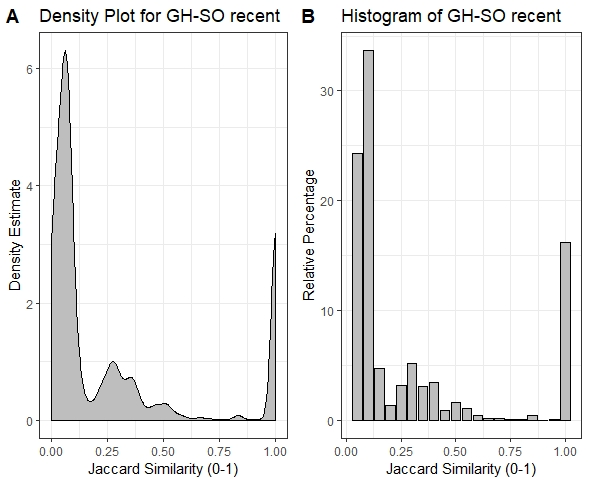
\includegraphics[width=\textwidth]{figures/GH_SO_recent.jpeg}\\
          \caption{Density Plot(A) and Histogram(B) of GH-recent and SO-recent data set comparison.}
          \label{fig:GH_SO_recent}
        \end{figure}
        
        Figure \ref{fig:GH_SO_recent} and \ref{fig:overlap_GH_SO_recent} show the results of comparing the most recent activity of users on GitHub and Stack Overflow. For the rest of the analysis this will be referred to as the \emph{GH-recent -- SO-recent} comparison. We chose Jaccard similarity as the similarity metric for this analysis, as we are interested in measuring the similarity between two sets of keywords for each user, coming from the \emph{GH-recent} and \emph{SO-recent} text corpora. Figure \ref{fig:GH_SO_recent} illustrates the distribution of the Jaccard similarity scores obtained from the \emph{GH-recent -- SO-recent} comparison. Plot A shows a density plot, while Plot B is a  histogram of the Jaccard similarity scores. The distribution from Figure \ref{fig:GH_SO_recent} shows that the majority of the population has very low Jaccard similarity scores, which means that there is a very low similarity between most user's \emph{GH-recent} and \emph{SO-recent} data. The histogram paints the clearest picture by showing that the highest relative percentage of Jaccard similarity scores are \{0, 0.05, 0.10 and 1\}.
        
        \begin{figure}
          % Requires 
          \centering
          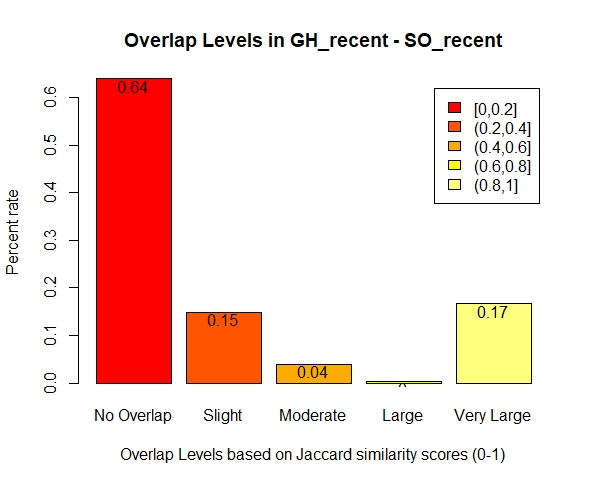
\includegraphics[width=\textwidth]{figures/overlap_GH_SO_recent.jpeg}\\
          \caption{Overlap levels between GH-recent and SO-recent data sets.}
          \label{fig:overlap_GH_SO_recent}
        \end{figure}
        
        Figure \ref{fig:overlap_GH_SO_recent} drives home this point by creating five non-overlapping sub-intervals of Jaccard similarity scores from the [0,1] range, classifying each sub-interval of values to a scale of \emph{No, Slight, Moderate, Large and Very Large Overlap}. When comparing the GH-recent -- SO-recent text corpora Figure \ref{fig:overlap_GH_SO_recent} shows that 64\% of the population has no overlap, 15\% has slight overlap, 4\% has moderate overlap, and 17\% has a very large overlap. 
        
        \begin{figure}
          % Requires 
          \centering
          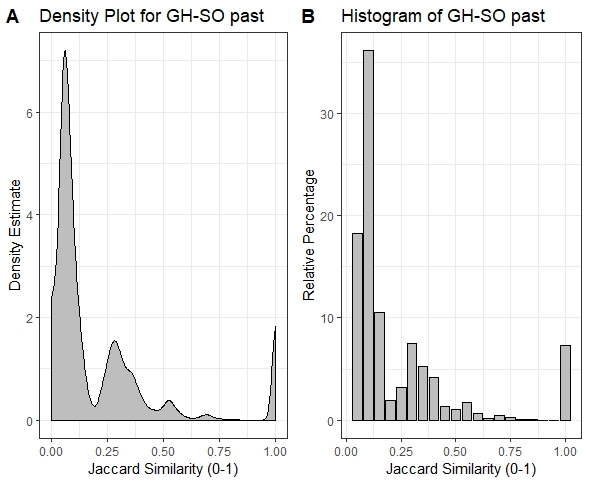
\includegraphics[width=\textwidth]{figures/GH_SO_past.jpeg}\\
          \caption{Density Plot(A) and Histogram(B) of GH-past and SO-past data set comparison.}
          \label{fig:GH_SO_past}
        \end{figure}
        
        Figure \ref{fig:GH_SO_past} and \ref{fig:overlap_GH_SO_past} show the results of comparing the past activity of users on GitHub and Stack Overflow. This will be referred to as the \emph{GH-past -- SO-past} comparison. Same as above, Jaccard similarity is the similarity metric chosen to measure the similarity between two sets of keywords for each user, coming from the \emph{GH-past} and \emph{SO-past} text corpora. Figure \ref{fig:GH_SO_past} illustrates the distribution of the Jaccard similarity scores obtained from the \emph{GH-past -- SO-past} comparison. Plot A shows a density plot, while Plot B is a  histogram of the Jaccard similarity scores. The distribution from Figure \ref{fig:GH_SO_past} is similar to the one from Figure \ref{fig:GH_SO_recent} and it shows that the majority of the population has very low Jaccard similarity scores. The density plot shows that most of the population has Jaccard similarity scores of \{0.05, 0.10, 0.15\}, while there are quite a few extreme scores of 0 and 1. This distribution suggests that there is a very low similarity between most user's expertise terms found in the \emph{GH-past} and \emph{SO-past} corpora. 
        
        \begin{figure}
          % Requires 
          \centering
          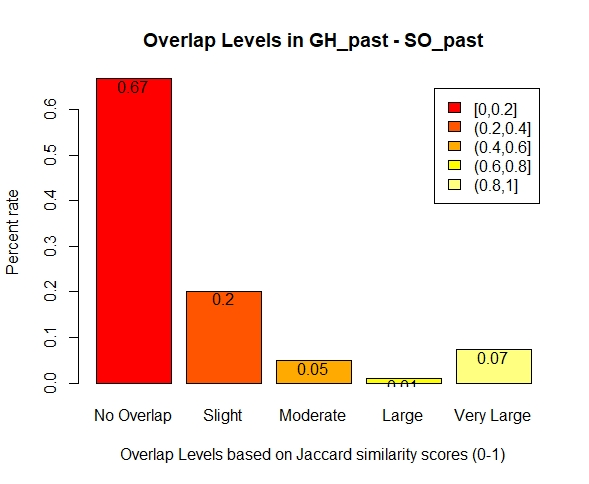
\includegraphics[width=\textwidth]{figures/overlap_SO_GH_past.jpeg}\\
          \caption{Overlap levels between GH-past and SO-past data sets.}
          \label{fig:overlap_GH_SO_past}
        \end{figure}
        
        Figure \ref{fig:overlap_GH_SO_past} confirms the findings above by considering the same five overlap levels as in Figure \ref{fig:overlap_GH_SO_recent}. When comparing the expertise terms in the GH-past - SO-past text corpora, Figure \ref{fig:overlap_GH_SO_past} shows that 67\% of the population has no overlap, 20\% has slight overlap, 5\% has moderate overlap, 1\% has large overlap, and 7\% has a very large overlap. \\
        
        \fbox{\begin{minipage}{5.5in}
            Answer to RQ2: The comparison of GH-recent and SO-recent text corpora showed that 64\% of the population have no overlap, while the GH-past and SO-past comparison concluded that 67\% of the population have no overlap. These results suggest that developers build different expertise profiles on GitHub and Stack Overflow.
        \end{minipage}}
    
    \section{Cross-platform Transferable Knowledge\label{sec:results_rq3}}
        % RQ3:  What knowledge is transferable from one platform to another?
        
        This section is concerned with discovering what knowledge is transferable from one platform to another. This question is answered by qualitatively analyzing the \emph{Top-$30$} most frequent common expertise terms for each user between the two platforms. For the experiment setup behind this analysis, we refer you to Section \ref{RQ3_task}.
        
        Table \ref{tab:RQ3_past} displays the frequencies of common expertise terms in the pair of \{GH-past, SO-past\} text corpora, while Table \ref{tab:RQ3_recent} presents the same kind of common expertise terms in the pair of \{GH-recent, SO-recent\} text corpora.
        
        \begin{table}
          \centering
          \caption{Most common words in GH-past and SO-past text corpora.}\label{tab:RQ3_past}
            \vspace{6pt} % Required to get proper spacing between caption and table
          \begin{tabular}{|c c c | c c c|}
            \hline
            Ranking & Keyword & Frequency & Ranking & Keyword & Frequency \\
            \hline\hline
            1 & library & 43,123 & 16 & base & 16,798 \\
            2 & code & 37,621 & 17 & implementation & 16,670 \\
            3 & simple & 32,762 & 18 & client & 15,833 \\
            4 & type & 30,948 & 19 & test & 15,723 \\
            5 & javascript & 30,044 & 20 & http & 15,674 \\
            6 & project & 26,255 & 21 & page & 15,423 \\
            7 & web & 25,083 & 22 & game & 13,890 \\
            8 & tool & 24,967 & 23 & website & 13,255 \\
            9 & https & 24,738 & 24 & package & 12,982 \\
            10 & file & 24,737 & 25 & repository & 11,690 \\
            11 & html & 22,333 & 26 & add & 11,421 \\
            12 & github & 21,317 & 27 & method & 11,421 \\
            13 & script & 20,318 & 28 & line & 11,252 \\
            14 & source & 20,266 & 29 & api & 11,144 \\
            15 & language & 19,855 & 30 & datum & 10,980 \\
            \hline
          \end{tabular}
        \end{table}
        
        In Table \ref{tab:RQ3_past} one can notice a general pattern of mostly web development related terms showing up in the \emph{Top-$30$} most frequent common expertise terms used in GH-past and SO-past text corpora. Examples of such terms include \emph{javascript, web, https, html, client, http, page, website}, and \emph{api}. Another noticeable trend is the source code and version control related keywords, such as \emph{library, code, project, tool, file, github, script, source, language, implementation, test, package, repository}, and \emph{method}. The first pattern could suggest that most common conversations in the GH-past and SO-past text corpora involve discussions about web development. The second pattern is intuitive, as both collaborative platforms contain source code and project related software artifacts, thus a possible knowledge transfer could occur by the cross-platform interaction of developers. 
        
        \begin{table}
          \centering
          \caption{Most common words in GH-recent and SO-recent text corpora.}\label{tab:RQ3_recent}
            \vspace{6pt} % Required to get proper spacing between caption and table
          \begin{tabular}{|c c c | c c c|}
            \hline
            Ranking & Keyword & Frequency & Ranking & Keyword & Frequency \\
            \hline\hline
            1 & test & 56,302 & 16 & heroku & 15,764 \\
            2 & simple & 51,226 & 17 & buildpack & 15,764 \\
            3 & library & 44,781 & 18 & cli & 15,764 \\
            4 & app & 43,750 & 19 & rb & 15,764 \\
            5 & api & 35,881 & 20 & activerecord & 15,764 \\
            6 & base & 26,075 & 21 & rspec & 15,764 \\
            7 & client & 25,381 & 22 & active & 15,764 \\
            8 & code & 22,052 & 23 & github & 15,297 \\
            9 & file & 21,538 & 24 & web & 12,890 \\
            10 & application & 19,620 & 25 & add & 12,849 \\
            11 & https & 16,764 & 26 & change & 12,849\\
            12 & ruby & 15,764  & 27 & remove & 12,849 \\
            13 & rail & 15,764 & 28 & check & 12,849\\
            14 & ember & 15,764 & 29 & make & 11,231 \\
            15 & gem & 15,764 & 30 & comment & 11,231\\
            \hline
          \end{tabular}
        \end{table}
        
        In Table \ref{tab:RQ3_recent} one can see the same general pattern of web development related terms dominated the \emph{Top-$30$} most frequent common expertise terms used in GH-recent and SO-recent text corpora, however, there is one noticeable discrepancy. In the \emph{recent} text corpora (containing data between 2016 and 2019) the list of common expertise terms have shifted towards \emph{Ruby and Heroku} related terms. Examples of this pattern include keywords like \emph{ruby, rail, gem, heroku, buildpack, rb, activerecord}, and \emph{rspec}. The web development pattern is also present in Table \ref{tab:RQ3_recent} by terms such as \emph{app, api, client, application, https, ember}, and \emph{web}. Finally, there is also a smaller cluster of source code and version control related keywords, such as \emph{test, library, code, file, github}, and \emph{comment}. These patterns suggest that most common conversations in GH-recent and SO-recent text corpora involve discussions about web development, source code, version control, and there might have been a popular trend in \emph{Ruby on Rails} discussions that the LDA model's topics detected more often than other programming language related discussions. 
        
        The co-occuring keywords in both Table \ref{tab:RQ3_past} and Table \ref{tab:RQ3_recent} are \emph{test, simple, library, api, base, client, code, file, https, github, web}, and \emph{add}. These keywords could be subjectively labelled as a combination of \emph{source code, GitHub and web development} related terms. \\
        
        \fbox{\begin{minipage}{5.5in}
            Answer to RQ3: Common expertise terms used in both GitHub and Stack Overflow text corpora suggest that \emph{source code, version control and web development} related skills are most transferable knowledge. 
        \end{minipage}}
    
    \section{Expertise Evolution\label{sec:results_rq4}}
        % RQ4: How does developer expertise evolve on Stack Overflow and GitHub?
        
        The \emph{Expertise Evolution Analysis} is concerned with comparing the evolution of expertise of the same users on Stack Overflow and GitHub. This analysis should answer the research question about how developer expertise changes over time on the two collaborative platforms. In this analysis, the change over time of GitHub and Stack Overflow text corpora are being analyzed. Two separate comparisons are considered: GH-past with GH-recent, and SO-past with SO-recent. For further details on the experiment setup behind this analysis see Section \ref{RQ4_task}.
        
        \begin{figure}
          % Requires 
          \centering
          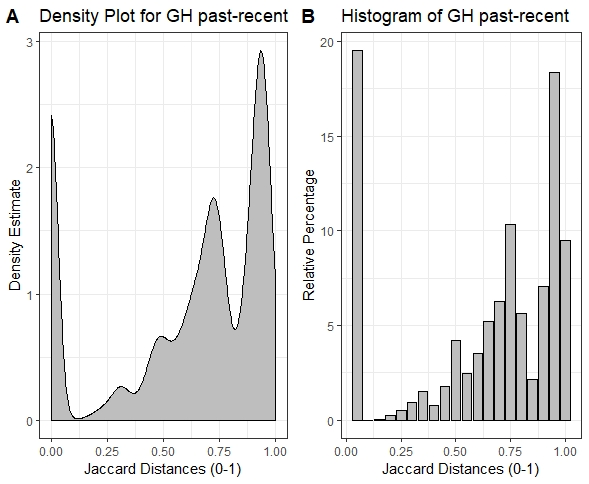
\includegraphics[width=\textwidth]{figures/GH_past-recent.jpeg}\\
          \caption{Density Plot(A) and Histogram(B) of GitHub past and recent data set comparison.}
          \label{fig:GH_past_recent}
        \end{figure}
        
        Figure \ref{fig:GH_past_recent} and Figure \ref{fig:change_GH_past_recent} show the results of comparing the past and recent activity of users on GitHub. For the rest of the analysis, this will be referred to as the \emph{GH past-recent} comparison. We chose \emph{Jaccard Distance} as the distance metric for this analysis, as we are interested in measuring the difference, thus distance (or dissimilarity) between two sets of keywords for each user, coming from the \emph{GH-past} and \emph{GH-recent} text corpora. 
        
        Figure \ref{fig:GH_past_recent} illustrates the distribution of the \emph{Jaccard Distance} scores obtained from the \emph{GH past-recent} comparison. Plot A shows a density plot, while Plot B is a histogram of the \emph{Jaccard Distance} scores. The distribution from Figure \ref{fig:GH_past_recent} shows that the majority of the population has very large \emph{Jaccard Distance} scores, which means that there is significant difference between most users' \emph{GH-past} and \emph{GH-recent} data. However, we can see on the histogram that there is a spike at \emph{Jaccard Distance} score of 0, meaning that there are some users who have the same expertise data in both \emph{GH-past} and \emph{GH-recent} text corpora.
        
        \begin{figure}
          % Requires 
          \centering
          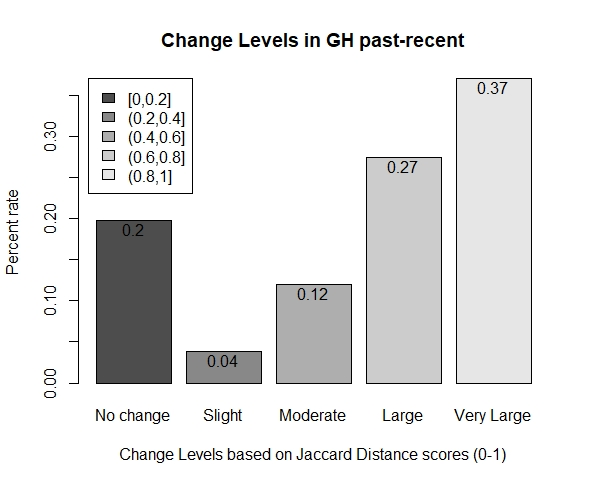
\includegraphics[width=\textwidth]{figures/change_level_GH_past-recent.jpeg}\\
          \caption{Change levels between GitHub past and recent data sets.}
          \label{fig:change_GH_past_recent}
        \end{figure}
        
        The distribution seen in Figure \ref{fig:GH_past_recent} suggests a diverse, mixed population of users between high and low \emph{Jaccard Distance} scores. Figure \ref{fig:change_GH_past_recent} should paint a more clear picture by creating five non-overlapping sub-intervals of \emph{Jaccard Distance} scores from the [0,1] range, classifying each sub-interval of values to a scale of \emph{No, Slight, Moderate, Large and Very Large Change}. The \emph{GH past-recent} comparison in Figure \ref{fig:change_GH_past_recent} shows that 20\% of the population has no change, 4\% has a slight change, 12\% has moderate change, 27\% has a large change, while 37\% has a very large change over time. This result concludes that most of the developer population has largely changed their expertise over time, however, 20\% of users maintain the same expertise profile on GitHub over time.
        
        \begin{figure}
          % Requires 
          \centering
          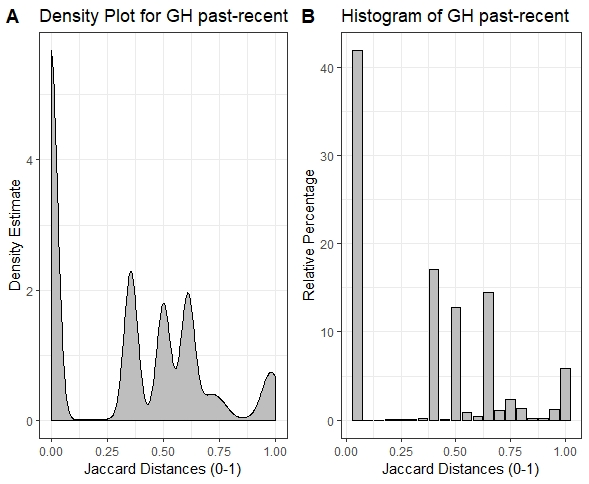
\includegraphics[width=\textwidth]{figures/SO_past-recent.jpeg}\\
          \caption{Density Plot(A) and Histogram(B) of Stack Overflow past and recent data set comparison.}
          \label{fig:SO_past_recent}
        \end{figure}
        
        Figure \ref{fig:SO_past_recent} and Figure \ref{fig:change_SO_past_recent} show the results of comparing the past and recent activity of users on Stack Overflow. For the rest of the analysis, this will be referred to as the \emph{SO past-recent} comparison. In this analysis, we are measuring the difference between two sets of keywords for each user coming from the \emph{SO-past} and \emph{SO-recent} text corpora, thus we use \emph{Jaccard Distance}. Figure \ref{fig:SO_past_recent} illustrates the distribution of the \emph{Jaccard Distance} scores obtained from the \emph{SO past-recent} comparison. Plot A is a density plot, while Plot B is a histogram of the \emph{Jaccard Distance} scores. 
         
        The distribution in Figure \ref{fig:SO_past_recent} shows many spikes at various \emph{Jaccard Distance} values, which shows a very specific behaviour. From the histogram it can be seen that the largest spike it at a value of 0, meaning that some users have the same expertise data in both \emph{SO-past} and \emph{SO-recent} text corpora. The second trend shows that some user activity comparison having the same \emph{Jaccard Distance} values of 0.40, 0.50 and 0.60, meaning that their more recent expertise differs from the past one.
        
        \begin{figure}
          % Requires 
          \centering
          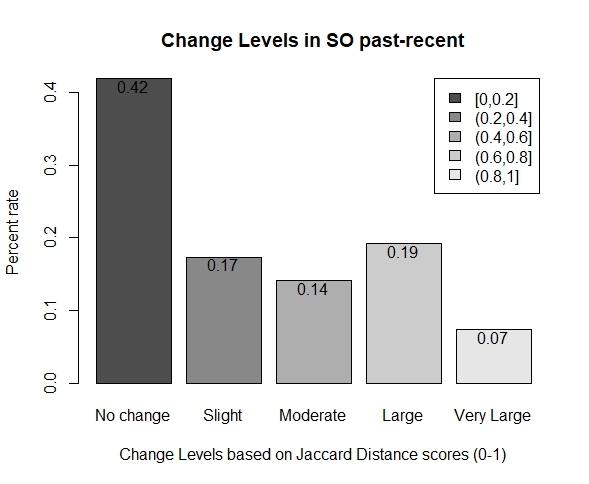
\includegraphics[width=\textwidth]{figures/change_levels_SO_past-recent.jpeg}\\
          \caption{Change levels between Stack Overflow past and recent data sets.}
          \label{fig:change_SO_past_recent}
        \end{figure}
        
        The distribution seen in Figure \ref{fig:SO_past_recent} suggests a diverse population of both high and low \emph{Jaccard Distance} scores. Figure \ref{fig:change_SO_past_recent} offers more details about the population by creating five non-overlapping sub-intervals of \emph{Jaccard Distance} scores, classifying each sub-interval of values to a scale of \emph{No, Slight, Moderate, Large and Very Large Change}. The \emph{SO past-recent} comparison in Figure \ref{fig:change_SO_past_recent} reveals that 42\% of the population has no change, 17\% has slight change, 14\% has moderate change, 19\% has a large change, while only 7\% has a very large change over time, thus concluding that most analyzed developer population on Stack Overflow has \emph{no, slight or moderate changes} in their expertise over time.
        
        \fbox{\begin{minipage}{5.5in}
            Answer to RQ4: The comparison of GH past-recent text corpora showed that 64\% of the analyzed population of developers has either large or very large changes in their expertise, concluding that most of the analyzed GitHub population has largely changed their expertise over time. For the comparison of SO past-recent text corpora, this is not the case, as 42\% of the population has no change, while 31\% of the population has either slight or moderate changes in their expertise, concluding that most of the analyzed Stack Overflow population did not or only slightly changed their expertise over time.
        \end{minipage}}\\
        
        All data sets used in this work are made publicly available on Zenodo\footnote{\url{https://zenodo.org/record/3696079}}. Currently, all source code that was used to obtain these results is hosted on a private GitHub repository \footnote{\url{https://github.com/norberte/Mining-StackOverflow-Github}}, but it will be made public after the publication of this work.